\chapter{La méiose et le brassage génétique}\label{ch:g12:meiosis-genetic-shuffling}

Deux parents, chacun avec 46 \omterm{def:g10:universal-dna:information}{chromosomes}, produisent un enfant à 46 ---
et non à 92. Quelque part entre le corps des parents et l'enfant, le
compte est divisé par deux, et il l'est d'une façon qui distribue à
chaque enfant une main qu'aucun frère ni aucune sœur n'a jamais tenue~:
les mêmes parents, quarante ans d'enfants, et pas deux semblables sauf
de vrais jumeaux. Cette réduction de moitié est une division
particulière, la \omterm{def:g12:meiosis-genetic-shuffling:meiosis}{méiose}~; la distribution est ce qu'elle fait des
\omterm{def:g10:universal-dna:information}{chromosomes} en chemin. Ce chapitre suit une \omterm{def:g10:cells-common-unit:cell}{cellule} à travers la
\omterm{def:g12:meiosis-genetic-shuffling:meiosis}{méiose}, compte les combinaisons qu'elle peut produire, et lit les
résultats de croisements qui révèlent, de l'extérieur, ce qui s'est
passé à l'intérieur.

\section{Diviser le jeu par deux}

\begin{definition}[Diploïde, haploïde, méiose]\label{def:g12:meiosis-genetic-shuffling:meiosis}
Une \omterm{def:g10:cells-common-unit:cell}{cellule} qui porte deux exemplaires de chaque \omterm{def:g11:cell-cycle-mitosis:chromosome}{chromosome} --- un de
chaque parent, les deux formant une paire de
\emph{chromosomes homologues} --- est
\emph{diploïde}\index{diploïde}, ce que l'on note $2n$ ($2n = 46$ chez
l'humain). Une \omterm{def:g10:cells-common-unit:cell}{cellule} qui n'en porte qu'un exemplaire est
\emph{haploïde}\index{haploïde}, ce que l'on note $n$. La
\emph{méiose}\index{méiose} est la suite de deux divisions par laquelle
une \omterm{def:g10:cells-common-unit:cell}{cellule} diploïde, après une seule réplication de son \omterm{def:g10:universal-dna:information}{ADN}, produit
quatre \omterm{def:g10:cells-common-unit:cell}{cellules} haploïdes --- les gamètes, ou leurs précurseurs. La
\emph{fécondation} unit deux gamètes haploïdes et rétablit le nombre
diploïde~: l'alternance de la méiose et de la fécondation est le cycle
de toute \omterm{def:g10:biodiversity-scales:species}{espèce} à reproduction sexuée.
\end{definition}

\begin{proposition}[Les deux divisions]\label{prop:g12:meiosis-genetic-shuffling:divisions}
Avant la \omterm{def:g12:meiosis-genetic-shuffling:meiosis}{méiose}, l'\omterm{def:g10:universal-dna:information}{ADN} est répliqué~: chaque \omterm{def:g11:cell-cycle-mitosis:chromosome}{chromosome} a deux
\omterm{def:g11:cell-cycle-mitosis:chromosome}{chromatides}. Ensuite~:
\begin{itemize}
  \item \emph{Première division} (\omterm{def:g12:meiosis-genetic-shuffling:meiosis}{méiose} I, \emph{réductionnelle})~:
        les chromosomes homologues s'apparient, deux à deux, sur
        l'équateur~; les membres de chaque paire sont tirés vers des
        pôles opposés. Chaque \omterm{def:g10:cells-common-unit:cell}{cellule} fille reçoit \emph{un \omterm{def:g11:cell-cycle-mitosis:chromosome}{chromosome}
        de chaque paire}, encore fait de deux \omterm{def:g11:cell-cycle-mitosis:chromosome}{chromatides}~: $n$
        \omterm{def:g10:universal-dna:information}{chromosomes}, quantité d'\omterm{def:g10:universal-dna:information}{ADN} $q$ (celle d'une \omterm{def:g10:cells-common-unit:cell}{cellule} \omterm{def:g12:meiosis-genetic-shuffling:meiosis}{diploïde}
        avant réplication).
  \item \emph{Seconde division} (\omterm{def:g12:meiosis-genetic-shuffling:meiosis}{méiose} II, \emph{équationnelle})~:
        comme une \omterm{def:g11:cell-cycle-mitosis:cycle}{mitose}, les \omterm{def:g11:cell-cycle-mitosis:chromosome}{chromatides} de chaque \omterm{def:g11:cell-cycle-mitosis:chromosome}{chromosome} se
        séparent. Chacune des quatre \omterm{def:g10:cells-common-unit:cell}{cellules} reçoit $n$ \omterm{def:g10:universal-dna:information}{chromosomes} à
        une \omterm{def:g11:cell-cycle-mitosis:chromosome}{chromatide}, quantité d'\omterm{def:g10:universal-dna:information}{ADN} $q/2$.
\end{itemize}
La première division divise par deux le nombre de \omterm{def:g10:universal-dna:information}{chromosomes}~; la
seconde ramène la quantité d'\omterm{def:g10:universal-dna:information}{ADN} à une \omterm{def:g11:cell-cycle-mitosis:chromosome}{chromatide} par \omterm{def:g11:cell-cycle-mitosis:chromosome}{chromosome}.
\end{proposition}
\admitted

\begin{omfigure}
\begin{tikzpicture}[font=\small, line cap=round]
  \tikzset{cellb/.style={draw, thick, fill=omDef!5, rounded corners=9pt, minimum width=2.5cm, minimum height=2.5cm},
           ma/.style={line width=3pt, omDef!80}, mb/.style={line width=3pt, omThm!80},
           mA/.style={line width=3pt, omDef!35}, mB/.style={line width=3pt, omThm!35}, cen/.style={fill=black}}
  % panel 1: diploid cell after S: two pairs (long pair blue, short pair red); paternal dark, maternal pale
  \begin{scope}
    \node[cellb] at (0,0) {};
    \draw[ma] (-0.75,0.7) .. controls (-0.62,0.1) .. (-0.75,-0.5); \draw[ma] (-0.49,0.7) .. controls (-0.62,0.1) .. (-0.49,-0.5); \fill[cen] (-0.62,0.1) circle (1.6pt);
    \draw[mA] (-0.2,0.7) .. controls (-0.07,0.1) .. (-0.2,-0.5); \draw[mA] (0.06,0.7) .. controls (-0.07,0.1) .. (0.06,-0.5); \fill[cen] (-0.07,0.1) circle (1.6pt);
    \draw[mb] (0.4,0.45) .. controls (0.53,0.1) .. (0.4,-0.25); \draw[mb] (0.66,0.45) .. controls (0.53,0.1) .. (0.66,-0.25); \fill[cen] (0.53,0.1) circle (1.6pt);
    \draw[mB] (0.9,0.45) .. controls (1.03,0.1) .. (0.9,-0.25); \draw[mB] (1.16,0.45) .. controls (1.03,0.1) .. (1.16,-0.25); \fill[cen] (1.03,0.1) circle (1.6pt);
    \node[anchor=north, align=center, font=\scriptsize, text width=3.05cm] at (0,-1.35) {après réplication~:\\ $2n = 4$, ADN $2q$};
  \end{scope}
  % panel 2: metaphase I: pairs on the equator
  \begin{scope}[xshift=3.2cm]
    \node[cellb] at (0,0) {};
    \draw[dashed, gray] (-1.1,0) -- (1.1,0);
    \draw[ma] (-0.7,0.55) .. controls (-0.57,0.1) .. (-0.7,-0.35); \draw[ma] (-0.44,0.55) .. controls (-0.57,0.1) .. (-0.44,-0.35); \fill[cen] (-0.57,0.15) circle (1.6pt);
    \draw[mA] (-0.7,-0.05) .. controls (-0.57,-0.5) .. (-0.7,-0.95); \draw[mA] (-0.44,-0.05) .. controls (-0.57,-0.5) .. (-0.44,-0.95); \fill[cen] (-0.57,-0.15) circle (1.6pt);
    \draw[mb] (0.45,0.5) .. controls (0.58,0.2) .. (0.45,-0.1); \draw[mb] (0.71,0.5) .. controls (0.58,0.2) .. (0.71,-0.1); \fill[cen] (0.58,0.15) circle (1.6pt);
    \draw[mB] (0.45,0.1) .. controls (0.58,-0.2) .. (0.45,-0.5); \draw[mB] (0.71,0.1) .. controls (0.58,-0.2) .. (0.71,-0.5); \fill[cen] (0.58,-0.15) circle (1.6pt);
    \node[anchor=north, align=center, font=\scriptsize, text width=3.05cm] at (0,-1.35) {méiose I~: paires\\ d'homologues à l'équateur};
  \end{scope}
  % panel 3: two cells after MI, each n=2 with two chromatids
  \begin{scope}[xshift=6.4cm]
    \node[cellb, minimum height=1.15cm] at (0,0.7) {};
    \node[cellb, minimum height=1.15cm] at (0,-0.7) {};
    \draw[ma] (-0.55,1.15) .. controls (-0.42,0.7) .. (-0.55,0.25); \draw[ma] (-0.29,1.15) .. controls (-0.42,0.7) .. (-0.29,0.25); \fill[cen] (-0.42,0.7) circle (1.6pt);
    \draw[mB] (0.35,1.0) .. controls (0.48,0.7) .. (0.35,0.4); \draw[mB] (0.61,1.0) .. controls (0.48,0.7) .. (0.61,0.4); \fill[cen] (0.48,0.7) circle (1.6pt);
    \draw[mA] (-0.55,-0.25) .. controls (-0.42,-0.7) .. (-0.55,-1.15); \draw[mA] (-0.29,-0.25) .. controls (-0.42,-0.7) .. (-0.29,-1.15); \fill[cen] (-0.42,-0.7) circle (1.6pt);
    \draw[mb] (0.35,-0.4) .. controls (0.48,-0.7) .. (0.35,-1.0); \draw[mb] (0.61,-0.4) .. controls (0.48,-0.7) .. (0.61,-1.0); \fill[cen] (0.48,-0.7) circle (1.6pt);
    \node[anchor=north, align=center, font=\scriptsize, text width=3.05cm] at (0,-1.35) {deux cellules~: $n = 2$,\\ deux chromatides, ADN $q$};
  \end{scope}
  % panel 4: four cells after MII, single chromatids
  \begin{scope}[xshift=9.6cm]
    \foreach \y in {1.05,0.35,-0.35,-1.05} \node[cellb, minimum height=0.6cm, minimum width=2.3cm] at (0,\y) {};
    \draw[ma] (-0.5,1.3) -- (-0.5,0.8); \fill[cen] (-0.5,1.05) circle (1.4pt); \draw[mB] (0.4,1.22) -- (0.4,0.88); \fill[cen] (0.4,1.05) circle (1.4pt);
    \draw[ma] (-0.5,0.6) -- (-0.5,0.1); \fill[cen] (-0.5,0.35) circle (1.4pt); \draw[mB] (0.4,0.52) -- (0.4,0.18); \fill[cen] (0.4,0.35) circle (1.4pt);
    \draw[mA] (-0.5,-0.1) -- (-0.5,-0.6); \fill[cen] (-0.5,-0.35) circle (1.4pt); \draw[mb] (0.4,-0.18) -- (0.4,-0.52); \fill[cen] (0.4,-0.35) circle (1.4pt);
    \draw[mA] (-0.5,-0.8) -- (-0.5,-1.3); \fill[cen] (-0.5,-1.05) circle (1.4pt); \draw[mb] (0.4,-0.88) -- (0.4,-1.22); \fill[cen] (0.4,-1.05) circle (1.4pt);
    \node[anchor=north, align=center, font=\scriptsize, text width=3.05cm] at (0,-1.45) {quatre gamètes~: $n = 2$,\\ une chromatide, ADN $q/2$};
  \end{scope}
\end{tikzpicture}

{\small La \omterm{def:g12:meiosis-genetic-shuffling:meiosis}{méiose} dans une \omterm{def:g10:cells-common-unit:cell}{cellule} à deux paires de \omterm{def:g10:universal-dna:information}{chromosomes}
($2n = 4$)~; les teintes foncées et pâles marquent les deux membres de
chaque paire, venus des deux parents. La première division sépare les
homologues, la seconde les \omterm{def:g11:cell-cycle-mitosis:chromosome}{chromatides}. Ici, le long \omterm{def:g11:cell-cycle-mitosis:chromosome}{chromosome} foncé
est parti avec le court \omterm{def:g11:cell-cycle-mitosis:chromosome}{chromosome} pâle~: l'une des deux distributions
possibles.}
\end{omfigure}

\begin{omfigure}
\begin{tikzpicture}
\begin{axis}[
  width=0.88\linewidth, height=5.2cm,
  axis x line=bottom, axis y line=left,
  xmin=0, xmax=10, ymin=0, ymax=2.7,
  xlabel={temps}, ylabel={ADN par cellule},
  xlabel style={font=\small, at={(axis description cs:0.5,-0.1)}, anchor=north},
  ylabel style={font=\small},
  tick label style={font=\small}, xtick=\empty,
  ytick={0.5,1,2}, yticklabels={$q/2$, $q$, $2q$},
  clip=false,
]
\addplot[thick, omDef] coordinates {(0,1) (2,1) (4,2) (5.9,2) (6,1) (7.9,1) (8,0.5) (10,0.5)};
\draw[dashed, gray] (axis cs:2,0) -- (axis cs:2,2.2); \draw[dashed, gray] (axis cs:4,0) -- (axis cs:4,2.2);
\draw[dashed, gray] (axis cs:6,0) -- (axis cs:6,2.2); \draw[dashed, gray] (axis cs:8,0) -- (axis cs:8,2.2);
\node[font=\small, anchor=south] at (axis cs:1,2.25) {$2n$, $q$};
\node[font=\small, anchor=south] at (axis cs:3,2.25) {phase S};
\node[font=\small, anchor=south] at (axis cs:5,2.25) {$2n$, $2q$};
\node[font=\small, anchor=south, omThm] at (axis cs:6,2.45) {méiose I};
\node[font=\small, anchor=south] at (axis cs:7,2.25) {$n$, $q$};
\node[font=\small, anchor=south, omThm] at (axis cs:8,2.45) {méiose II};
\node[font=\small, anchor=south] at (axis cs:9,2.25) {$n$, $q/2$};
\end{axis}
\end{tikzpicture}

{\small L'\omterm{def:g10:universal-dna:information}{ADN} par \omterm{def:g10:cells-common-unit:cell}{cellule} au cours de la \omterm{def:g12:meiosis-genetic-shuffling:meiosis}{méiose}. Une réplication, puis
deux divisions sans réplication entre elles~: les gamètes détiennent le
quart de l'\omterm{def:g10:universal-dna:information}{ADN} que la \omterm{def:g10:cells-common-unit:cell}{cellule} mère détenait après S, et la moitié de ce
que détient une \omterm{def:g10:cells-common-unit:cell}{cellule} \omterm{def:g12:meiosis-genetic-shuffling:meiosis}{diploïde} au repos.}
\end{omfigure}

\begin{example}[Les nombres humains]\label{ex:g12:meiosis-genetic-shuffling:numbers}
Une \omterm{def:g10:cells-common-unit:cell}{cellule} germinale du testicule, $2n = 46$, se réplique en 46
\omterm{def:g10:universal-dna:information}{chromosomes} à deux \omterm{def:g11:cell-cycle-mitosis:chromosome}{chromatides} ($2q$)~; après la \omterm{def:g12:meiosis-genetic-shuffling:meiosis}{méiose} I, deux
\omterm{def:g10:cells-common-unit:cell}{cellules} à 23 \omterm{def:g10:universal-dna:information}{chromosomes} à deux \omterm{def:g11:cell-cycle-mitosis:chromosome}{chromatides} ($q$)~; après la \omterm{def:g12:meiosis-genetic-shuffling:meiosis}{méiose}
II, quatre spermatozoïdes à 23 \omterm{def:g10:universal-dna:information}{chromosomes} à une \omterm{def:g11:cell-cycle-mitosis:chromosome}{chromatide} ($q/2$). À
la fécondation, $23 + 23 =
46$ et $q/2 + q/2 = q$~: le zygote retrouve l'état d'une \omterm{def:g10:cells-common-unit:cell}{cellule}
\omterm{def:g12:meiosis-genetic-shuffling:meiosis}{diploïde} au repos. Dans l'ovaire, les mêmes divisions produisent un
gros ovocyte et trois \omterm{def:g10:cells-common-unit:cell}{cellules} minuscules qui sont éliminées~;
l'arithmétique est identique.
\end{example}

\section{Le brassage}

\begin{proposition}[Le brassage interchromosomique]\label{prop:g12:meiosis-genetic-shuffling:assortment}
À la métaphase I, chaque paire d'homologues se place sur l'équateur
indépendamment des autres paires~: quel membre d'une paire gagne quel
pôle est décidé par le hasard, paire par paire. Une \omterm{def:g10:cells-common-unit:cell}{cellule} à $n$
paires peut donc produire $2^n$ combinaisons différentes de \omterm{def:g10:universal-dna:information}{chromosomes}
paternels et maternels dans ses gamètes --- $2^{23} \approx \num{8.4e6}$
chez l'humain. La fécondation, qui unit au hasard deux
gamètes de ce genre, donne $2^{23}
\times 2^{23} \approx \num{7e13}$ combinaisons de \omterm{def:g10:universal-dna:information}{chromosomes} pour les
enfants d'un même couple, avant même de compter toute autre source de
variété.
\end{proposition}
\admitted

\begin{proposition}[Le crossing-over]\label{prop:g12:meiosis-genetic-shuffling:crossingover}
Tandis que les homologues sont appariés, tôt dans la \omterm{def:g12:meiosis-genetic-shuffling:meiosis}{méiose} I, deux
\omterm{def:g11:cell-cycle-mitosis:chromosome}{chromatides} non sœurs se rompent au même point et se ressoudent en
croix~: c'est un \emph{crossing-over}\index{crossing-over}. Chaque
\omterm{def:g11:cell-cycle-mitosis:chromosome}{chromatide}, au-delà du point d'échange, porte désormais les \omterm{def:g10:universal-dna:gene}{allèles} de
l'homologue d'en face. Les \omterm{def:g10:universal-dna:information}{chromosomes} qui atteignent les gamètes ne
sont donc pas les \omterm{def:g10:universal-dna:information}{chromosomes} des parents mais des \omterm{def:g10:universal-dna:information}{chromosomes}
\emph{recombinés}, qui mêlent sur leur longueur les \omterm{def:g10:universal-dna:gene}{allèles} reçus des
deux grands-parents. Un à trois échanges se produisent sur chaque paire
à chaque \omterm{def:g12:meiosis-genetic-shuffling:meiosis}{méiose}, à des positions variables~: le nombre de gamètes
possibles est, en pratique, illimité.
\end{proposition}
\begin{proof}[Faits expérimentaux]
Au microscope, les homologues appariés de la \omterm{def:g12:meiosis-genetic-shuffling:meiosis}{méiose} I montrent des
points de croisement, les \emph{chiasmas}, où deux \omterm{def:g11:cell-cycle-mitosis:chromosome}{chromatides} changent
visiblement de partenaire. Les croisements où deux \omterm{def:g10:universal-dna:gene}{gènes} sont portés
par le même \omterm{def:g11:cell-cycle-mitosis:chromosome}{chromosome} donnent, dans la descendance, une minorité qui
porte des combinaisons nouvelles des \omterm{def:g10:universal-dna:gene}{allèles} des deux \omterm{def:g10:universal-dna:gene}{gènes} ---
combinaisons qu'aucun parent ne portait --- dans une proportion qui
dépend de la distance entre les \omterm{def:g10:universal-dna:gene}{gènes}~; des \omterm{def:g10:universal-dna:gene}{gènes} très éloignés sur un
\omterm{def:g11:cell-cycle-mitosis:chromosome}{chromosome} se recombinent aussi souvent que des \omterm{def:g10:universal-dna:gene}{gènes} portés par des
\omterm{def:g10:universal-dna:information}{chromosomes} différents. Des marqueurs moléculaires suivis dans des
familles montrent les segments de chaque \omterm{def:g11:cell-cycle-mitosis:chromosome}{chromosome} passant d'une
origine grand-parentale à l'autre en un ou deux points par \omterm{def:g11:cell-cycle-mitosis:chromosome}{chromosome}
et par génération.
\end{proof}

\begin{omfigure}
\begin{tikzpicture}[font=\small, line cap=round, >=Stealth]
  \tikzset{p/.style={line width=4pt, omDef!80}, m/.style={line width=4pt, omThm!70}}
  % before: two homologues, each two chromatids; alleles A/a, B/b
  \draw[p] (0,0) -- (0,3); \draw[p] (0.35,0) -- (0.35,3);
  \draw[m] (0.9,0) -- (0.9,3); \draw[m] (1.25,0) -- (1.25,3);
  \foreach \x in {0,0.35} { \node[font=\scriptsize, anchor=east, xshift=-1pt] at (\x,2.6) {}; }
  \node[font=\scriptsize, omDef!80!black, anchor=east] at (-0.15,2.6) {$A$};
  \node[font=\scriptsize, omDef!80!black, anchor=east] at (-0.15,0.5) {$B$};
  \node[font=\scriptsize, omThm!80!black, anchor=west] at (1.4,2.6) {$a$};
  \node[font=\scriptsize, omThm!80!black, anchor=west] at (1.4,0.5) {$b$};
  \node[anchor=north, align=center] at (0.62,-0.2) {homologues appariés\\ (deux chromatides chacun)};
  \draw[->, thick] (2.4,1.5) -- (3.4,1.5);
  % during: chiasma between the two inner chromatids at y=1.5
  \begin{scope}[xshift=4.2cm]
    \draw[p] (0,0) -- (0,3);
    \draw[p] (0.35,3) -- (0.35,1.6) -- (0.9,1.4) -- (0.9,0);
    \draw[m] (0.9,3) -- (0.9,1.6) -- (0.35,1.4) -- (0.35,0);
    \draw[m] (1.25,0) -- (1.25,3);
    \node[anchor=north, align=center] at (0.62,-0.2) {chiasma~: deux chromatides\\ se rompent et se ressoudent en croix};
  \end{scope}
  \draw[->, thick] (6.6,1.5) -- (7.6,1.5);
  % after: four chromatids separated
  \begin{scope}[xshift=8.4cm]
    \draw[p] (0,0) -- (0,3);
    \draw[p] (0.5,3) -- (0.5,1.5); \draw[m] (0.5,1.5) -- (0.5,0);
    \draw[m] (1.0,3) -- (1.0,1.5); \draw[p] (1.0,1.5) -- (1.0,0);
    \draw[m] (1.5,0) -- (1.5,3);
    \node[font=\scriptsize, anchor=south] at (0,3.05) {$AB$};
    \node[font=\scriptsize, anchor=south] at (0.5,3.05) {$Ab$};
    \node[font=\scriptsize, anchor=south] at (1.0,3.05) {$aB$};
    \node[font=\scriptsize, anchor=south] at (1.5,3.05) {$ab$};
    \node[anchor=north, align=center] at (0.75,-0.2) {quatre gamètes~: deux parentaux,\\ deux recombinés};
  \end{scope}
\end{tikzpicture}

{\small Un \omterm{prop:g12:meiosis-genetic-shuffling:crossingover}{crossing-over} entre deux \omterm{def:g10:universal-dna:gene}{gènes} $A$ et $B$ portés par le même
\omterm{def:g11:cell-cycle-mitosis:chromosome}{chromosome}. Deux des quatre \omterm{def:g11:cell-cycle-mitosis:chromosome}{chromatides} échangent leurs extrémités~;
des quatre gamètes, deux portent les combinaisons parentales ($AB$,
$ab$) et deux des combinaisons nouvelles ($Ab$, $aB$).}
\end{omfigure}

\begin{omfigure}
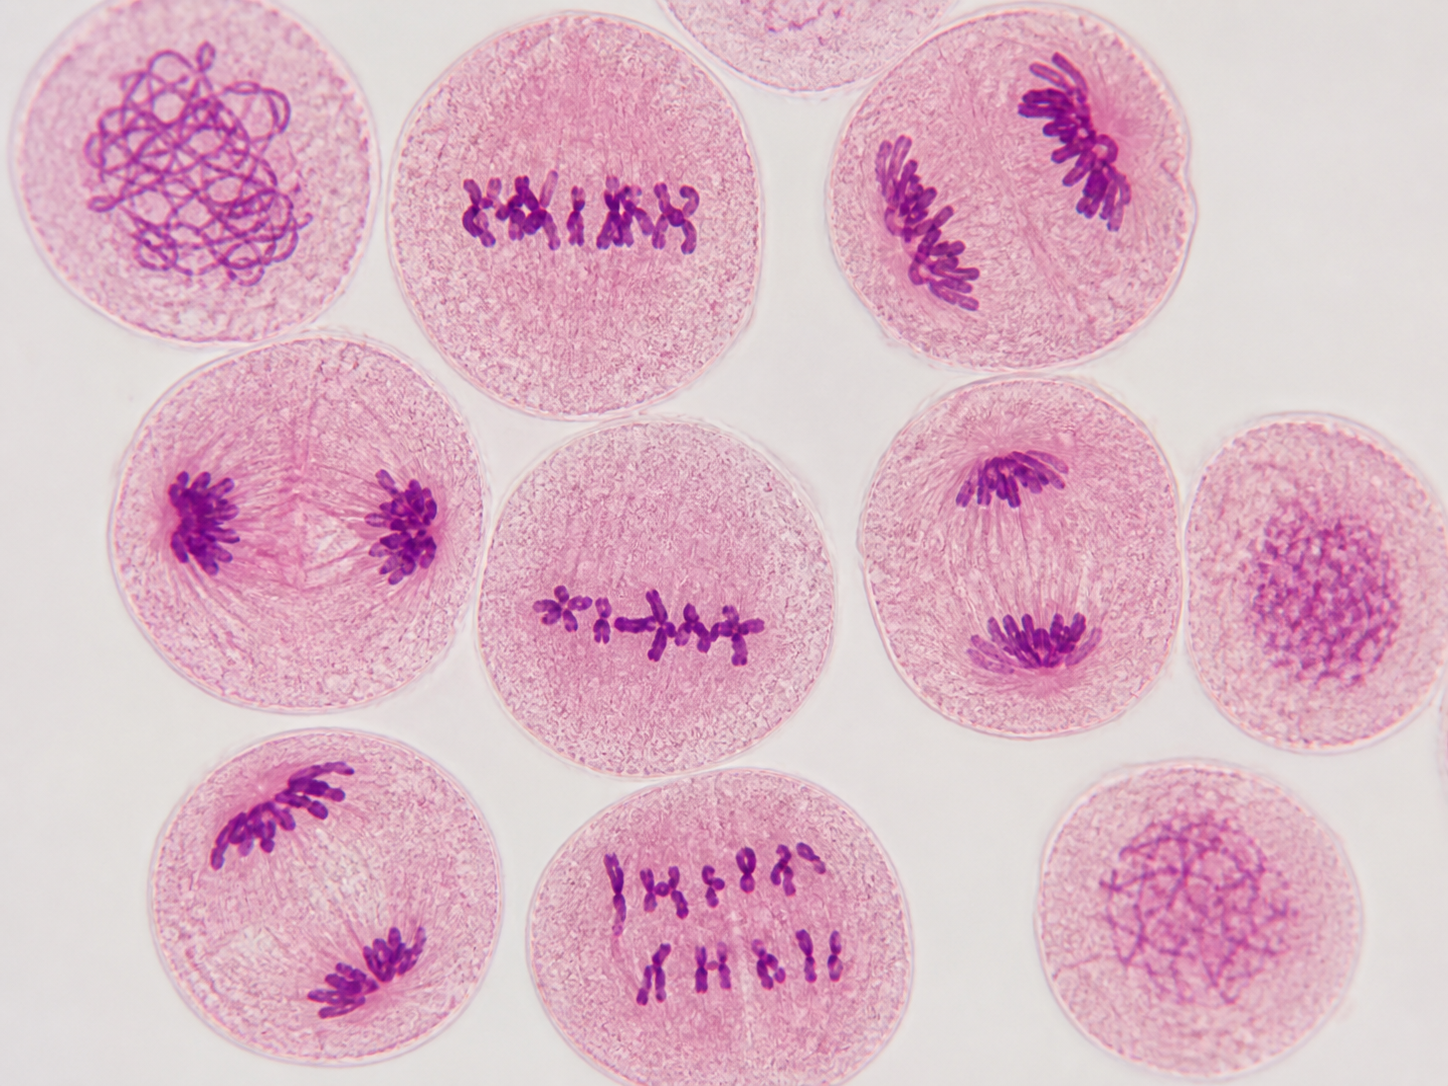
\includegraphics[width=0.56\linewidth]{images/book2/ai/g12-meiosis-lily-anther.png}

{\small Des \omterm{def:g10:cells-common-unit:cell}{cellules} d'anthère de lis en \omterm{def:g12:meiosis-genetic-shuffling:meiosis}{méiose}, colorées~: chez
certaines, les homologues appariés s'alignent en travers du milieu de
la \omterm{def:g10:cells-common-unit:cell}{cellule}~; chez d'autres, ils ont été tirés vers les deux pôles. Les
stades du schéma, vus dans le tissu qui fabrique le pollen.}
\end{omfigure}

\begin{example}[Trois sources de variété, dans l'ordre]\label{ex:g12:meiosis-genetic-shuffling:sources}
Un enfant de deux parents est neuf de trois façons~: le \omterm{prop:g12:meiosis-genetic-shuffling:crossingover}{crossing-over} a
rebâti chaque \omterm{def:g11:cell-cycle-mitosis:chromosome}{chromosome} de chaque gamète à partir des deux exemplaires
grand-parentaux~; le brassage interchromosomique a distribué dans le
gamète un \omterm{def:g11:cell-cycle-mitosis:chromosome}{chromosome} recombiné de chaque paire, parmi $2^{23}$
distributions~; la fécondation a joint un tel gamète à un autre tiré
des $2^{23}$ de l'autre parent. La \omterm{def:g11:mutations:mutation}{mutation}, qui a créé les \omterm{def:g10:universal-dna:gene}{allèles} que
l'on brasse, agit à une échelle de temps bien plus lente~: c'est le
brassage qui rend chaque génération neuve avec le même jeu de cartes.
\end{example}

\section{Lire le brassage dans un croisement}

\begin{omfigure}
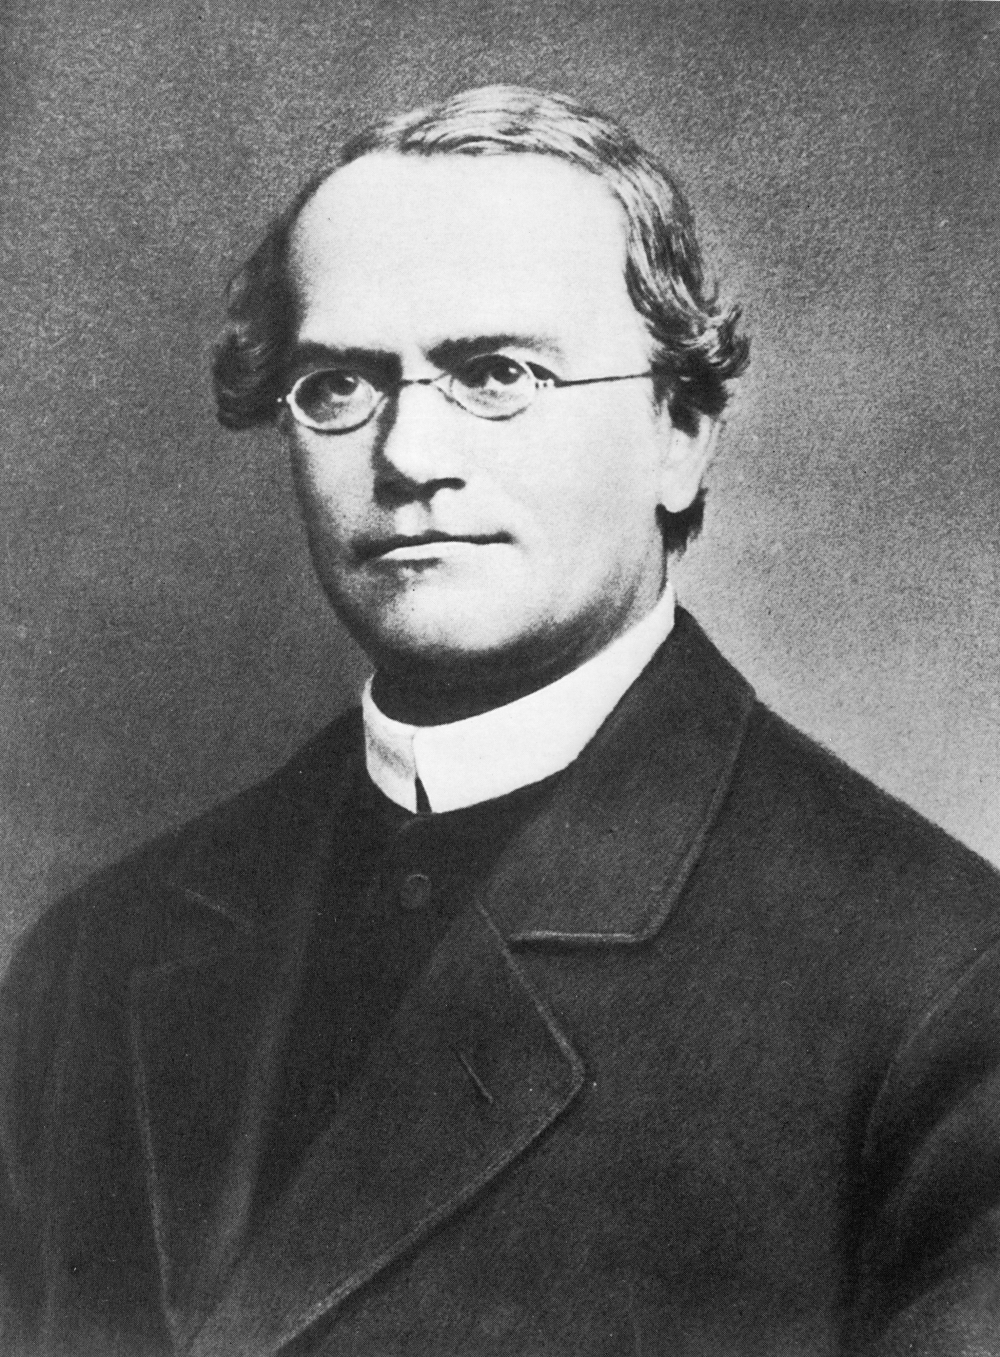
\includegraphics[width=0.3\linewidth]{images/book2/mendel.jpg}

{\small Gregor Mendel, qui a compté la descendance de croisements de pois dans un jardin de monastère dans les années 1860 et y a trouvé les rapports --- 3:1 pour un caractère, 9:3:3:1 pour deux --- que produit la \omterm{def:g12:meiosis-genetic-shuffling:meiosis}{méiose}, qu'il ignorait. Photographie, domaine public.}
\end{omfigure}

\begin{method}[Le croisement-test]\label{met:g12:meiosis-genetic-shuffling:testcross}
Pour voir quels gamètes fabrique un individu, on le croise avec un
partenaire ne portant que des \omterm{def:g10:universal-dna:gene}{allèles} \omterm{def:g11:genes-and-disease:genetic}{récessifs} (un
\emph{croisement-test})~: chaque descendant montre alors exactement les
\omterm{def:g10:universal-dna:gene}{allèles} que portait le gamète du parent testé. Pour deux \omterm{def:g10:universal-dna:gene}{gènes}, le
parent testé étant $AaBb$ et le partenaire $aabb$~:
\begin{enumerate}
  \item Compter les quatre sortes de descendants~: $AB$, $Ab$, $aB$,
        $ab$ (chacun portant aussi $ab$ venu du partenaire).
  \item Si les quatre sont également fréquents ($1:1:1:1$), les \omterm{def:g10:universal-dna:gene}{gènes}
        sont sur des \omterm{def:g10:universal-dna:information}{chromosomes} différents et se distribuent
        indépendamment.
  \item Si deux sortes (les combinaisons parentales) sont bien plus
        fréquentes que les deux autres (les recombinées), les \omterm{def:g10:universal-dna:gene}{gènes} sont
        sur le même \omterm{def:g11:cell-cycle-mitosis:chromosome}{chromosome}~; les recombinés viennent d'un
        \omterm{prop:g12:meiosis-genetic-shuffling:crossingover}{crossing-over}, et leur proportion mesure la distance entre les
        \omterm{def:g10:universal-dna:gene}{gènes}.
  \item Les recombinés sont toujours minoritaires et toujours en deux
        classes égales~; les parentaux également.
\end{enumerate}
\end{method}

\begin{example}[Deux croisements chez la drosophile]\label{ex:g12:meiosis-genetic-shuffling:fly}
Mouche A, hétérozygote pour la couleur du corps et la forme des ailes,
soumise à un croisement-test~: 254 gris-normales, 248
noires-vestigiales, 251 grises-vestigiales, 247 noires-normales ---
quatre classes égales, les \omterm{def:g10:universal-dna:gene}{gènes} sont sur des \omterm{def:g10:universal-dna:information}{chromosomes} différents.
Mouche B, hétérozygote pour la couleur du corps et celle des \omterm{def:g11:the-eye:parts}{yeux}~: 412
grises-rouges, 405 noires-pourpres, 44 grises-pourpres, 39
noires-rouges --- deux classes parentales d'environ 45~\% chacune et
deux classes recombinées d'environ 5~\%~: les \omterm{def:g10:universal-dna:gene}{gènes} sont sur le même
\omterm{def:g11:cell-cycle-mitosis:chromosome}{chromosome}, proches l'un de l'autre, séparés par un \omterm{prop:g12:meiosis-genetic-shuffling:crossingover}{crossing-over} dans
9~\% des \omterm{def:g12:meiosis-genetic-shuffling:meiosis}{méioses}.
\end{example}

\begin{omfigure}
\begin{tikzpicture}[font=\small]
  \draw[thick] (0,0) grid[step=1.4] (5.6,1.4);
  \node[fill=omDef!15, minimum width=1.3cm, minimum height=1.3cm, align=center] at (0.7,0.7) {$AB$\\ 254};
  \node[fill=omDef!15, minimum width=1.3cm, minimum height=1.3cm, align=center] at (2.1,0.7) {$Ab$\\ 251};
  \node[fill=omDef!15, minimum width=1.3cm, minimum height=1.3cm, align=center] at (3.5,0.7) {$aB$\\ 247};
  \node[fill=omDef!15, minimum width=1.3cm, minimum height=1.3cm, align=center] at (4.9,0.7) {$ab$\\ 248};
  \node[anchor=south] at (2.8,1.5) {mouche A~: gènes indépendants, $1:1:1:1$};
  \begin{scope}[xshift=7.4cm]
    \draw[thick] (0,0) grid[step=1.4] (5.6,1.4);
    \node[fill=omProp!25, minimum width=1.3cm, minimum height=1.3cm, align=center] at (0.7,0.7) {$AB$\\ 412};
    \node[fill=omThm!20, minimum width=1.3cm, minimum height=1.3cm, align=center] at (2.1,0.7) {$Ab$\\ 44};
    \node[fill=omThm!20, minimum width=1.3cm, minimum height=1.3cm, align=center] at (3.5,0.7) {$aB$\\ 39};
    \node[fill=omProp!25, minimum width=1.3cm, minimum height=1.3cm, align=center] at (4.9,0.7) {$ab$\\ 405};
    \node[anchor=south] at (2.8,1.5) {mouche B~: gènes liés, parentaux $\gg$ recombinés};
  \end{scope}
\end{tikzpicture}

{\small Les gamètes de deux mouches hétérozygotes, lus dans des
croisements-tests. Des classes égales signifient un brassage
indépendant~; deux grandes classes et deux petites signifient que les
\omterm{def:g10:universal-dna:gene}{gènes} sont liés, les petites classes étant produites par le
\omterm{prop:g12:meiosis-genetic-shuffling:crossingover}{crossing-over}.}
\end{omfigure}

\section{Quand le brassage se dérègle}

\begin{proposition}[Les erreurs de la méiose]\label{prop:g12:meiosis-genetic-shuffling:errors}
Il arrive qu'une paire d'homologues ne se sépare pas à la \omterm{def:g12:meiosis-genetic-shuffling:meiosis}{méiose} I, ou
deux \omterm{def:g11:cell-cycle-mitosis:chromosome}{chromatides} à la \omterm{def:g12:meiosis-genetic-shuffling:meiosis}{méiose} II~: un gamète reçoit deux exemplaires
d'un \omterm{def:g11:cell-cycle-mitosis:chromosome}{chromosome} et un autre aucun. Fécondés, ils donnent un zygote à
trois exemplaires (une \emph{trisomie}) ou à un seul (une
\emph{monosomie}). La plupart de ces zygotes ne se développent pas~;
ceux qui le font portent un ensemble de traits caractéristiques. La
trisomie 21 (environ une naissance sur 700) provoque un handicap
intellectuel et des malformations cardiaques, et c'est la plus
fréquente~; sa fréquence monte fortement avec l'âge de la mère. Un
\omterm{prop:g12:meiosis-genetic-shuffling:crossingover}{crossing-over} inégal --- des \omterm{def:g11:cell-cycle-mitosis:chromosome}{chromatides} échangeant des segments de
longueurs différentes --- produit un \omterm{def:g11:cell-cycle-mitosis:chromosome}{chromosome} à \omterm{def:g10:universal-dna:gene}{gène} dupliqué et un
autre à \omterm{def:g10:universal-dna:gene}{gène} délété~: le mécanisme par lequel les \omterm{def:g10:universal-dna:gene}{gènes} d'\omterm{def:g11:the-eye:photoreceptors}{opsines} du
\cref{ch:g11:the-eye} se sont multipliés, et par lequel naissent de
nouveaux \omterm{def:g10:universal-dna:gene}{gènes} (\cref{ch:g12:diversification-of-life}).
\end{proposition}
\admitted

\begin{omfigure}
\begin{tikzpicture}
\begin{axis}[
  width=0.84\linewidth, height=5.4cm,
  axis x line=bottom, axis y line=left,
  xmin=18, xmax=47, ymin=0, ymax=40,
  xlabel={âge de la mère (ans)}, ylabel={trisomies 21 pour 1000 naissances},
  xlabel style={font=\small, at={(axis description cs:0.5,-0.12)}, anchor=north},
  ylabel style={font=\small},
  tick label style={font=\small}, xtick={20,25,30,35,40,45}, ytick={0,10,20,30,40},
]
\addplot[thick, omThm, mark=*, mark size=1.5pt] coordinates
  {(20,0.7) (25,0.8) (30,1.1) (33,1.8) (35,2.9) (37,4.5) (39,7.5) (41,12) (43,20) (45,33)};
\end{axis}
\end{tikzpicture}

{\small Fréquence de la trisomie 21 à la naissance en fonction de l'âge
de la mère. Les ovocytes se forment avant la naissance d'une femme et
restent en pause en \omterm{def:g12:meiosis-genetic-shuffling:meiosis}{méiose} I pendant des décennies~; plus la pause est
longue, plus un défaut de séparation des homologues est probable.}
\end{omfigure}

\begin{example}[Chromosomes sexuels mal comptés]\label{ex:g12:meiosis-genetic-shuffling:sexchrom}
Un gamète sans \omterm{def:g11:cell-cycle-mitosis:chromosome}{chromosome} sexuel fécondé par un gamète \omterm{def:g11:genes-and-disease:genetic}{porteur} d'un X
donne un zygote XO~: une fille de petite taille dont les ovaires ne se
développent pas. Un ovocyte XX fécondé par un spermatozoïde Y donne
XXY~: un garçon dont les testicules restent petits et ne fabriquent pas
de spermatozoïdes. Dans les deux cas, \omterm{prop:g11:becoming-male-female:sry}{SRY} décide de la gonade comme au
\cref{ch:g11:becoming-male-female}~; c'est le nombre de \omterm{def:g10:universal-dna:information}{chromosomes} X
qui décide de l'essentiel du reste, et c'est pourquoi ce sont là les
plus bénignes des erreurs chromosomiques.
\end{example}

\begin{remark}[Pourquoi le sexe]\label{rem:g12:meiosis-genetic-shuffling:whysex}
Une bactérie se recopie~; un rosier peut naître d'une bouture. La
reproduction sexuée coûte plus cher --- deux parents, une \omterm{def:g12:meiosis-genetic-shuffling:meiosis}{méiose}, la
recherche d'un partenaire --- et son produit est un ensemble de
descendants tous différents de leurs parents et les uns des autres.
Cette différence est le but~: dans un environnement qui change, et face
à des parasites qui évoluent, une population d'individus variés a plus
de chances d'en contenir qui survivent qu'une population de copies. Le
brassage de ce chapitre est la matière première que la sélection des
deux chapitres suivants triera.
\end{remark}

\section{Exercices}

\begin{exercise}[$\star$]\label{exo:g12:meiosis-genetic-shuffling:1}
Définir \omterm{def:g12:meiosis-genetic-shuffling:meiosis}{diploïde} et \omterm{def:g12:meiosis-genetic-shuffling:meiosis}{haploïde}, et dire ce que la \omterm{def:g12:meiosis-genetic-shuffling:meiosis}{méiose} fait au nombre
de \omterm{def:g10:universal-dna:information}{chromosomes} et à la quantité d'\omterm{def:g10:universal-dna:information}{ADN}.
\end{exercise}

\begin{exercise}[$\star$]\label{exo:g12:meiosis-genetic-shuffling:2}
Qu'est-ce qui se sépare à la \omterm{def:g12:meiosis-genetic-shuffling:meiosis}{méiose} I~? À la \omterm{def:g12:meiosis-genetic-shuffling:meiosis}{méiose} II~? Quelle
division est la division réductionnelle~?
\end{exercise}

\begin{exercise}[$\star$]\label{exo:g12:meiosis-genetic-shuffling:3}
Une \omterm{def:g10:cells-common-unit:cell}{cellule} a $2n = 8$ et un \omterm{def:g10:universal-dna:information}{ADN} de $2q$ au début de la \omterm{def:g12:meiosis-genetic-shuffling:meiosis}{méiose}. Donner
le nombre de \omterm{def:g10:universal-dna:information}{chromosomes} et la quantité d'\omterm{def:g10:universal-dna:information}{ADN} des \omterm{def:g10:cells-common-unit:cell}{cellules} après la
\omterm{def:g12:meiosis-genetic-shuffling:meiosis}{méiose} I puis après la \omterm{def:g12:meiosis-genetic-shuffling:meiosis}{méiose} II.
\end{exercise}

\begin{exercise}[$\star$]\label{exo:g12:meiosis-genetic-shuffling:4}
Combien de combinaisons chromosomiques les gamètes d'une \omterm{def:g10:biodiversity-scales:species}{espèce} à
$2n = 8$ peuvent-ils montrer par le seul brassage interchromosomique~?
\end{exercise}

\begin{exercise}[$\star$]\label{exo:g12:meiosis-genetic-shuffling:5}
Qu'est-ce qu'un croisement-test, et que révèle la proportion de
descendants recombinés~?
\end{exercise}

\begin{exercise}[$\star\star$]\label{exo:g12:meiosis-genetic-shuffling:6}
D'après la figure de l'\omterm{def:g10:universal-dna:information}{ADN}, lire l'\omterm{def:g10:universal-dna:information}{ADN} par \omterm{def:g10:cells-common-unit:cell}{cellule} d'une \omterm{def:g10:cells-common-unit:cell}{cellule} en
\omterm{def:g12:meiosis-genetic-shuffling:meiosis}{méiose} I, d'une \omterm{def:g10:cells-common-unit:cell}{cellule} entre les deux divisions, et d'un gamète.
Expliquer pourquoi il n'y a pas de phase S entre les divisions.
\end{exercise}

\begin{exercise}[$\star\star$]\label{exo:g12:meiosis-genetic-shuffling:7}
Un croisement-test donne 300 $AB$, 298 $ab$, 302 $Ab$, 300 $aB$. Les
\omterm{def:g10:universal-dna:gene}{gènes} sont-ils liés~? Quels sont les gamètes du parent~?
\end{exercise}

\begin{exercise}[$\star\star$]\label{exo:g12:meiosis-genetic-shuffling:8}
Un croisement-test donne 460 $AB$, 455 $ab$, 42 $Ab$, 43 $aB$. Les
\omterm{def:g10:universal-dna:gene}{gènes} sont-ils liés~? Quelles classes sont recombinées, et quelle
fraction représentent-elles~?
\end{exercise}

\begin{exercise}[$\star\star$]\label{exo:g12:meiosis-genetic-shuffling:9}
Sur la figure du \omterm{prop:g12:meiosis-genetic-shuffling:crossingover}{crossing-over}, quels deux gamètes obtiendrait-on si
l'échange avait lieu \emph{au-dessus} des deux \omterm{def:g10:universal-dna:gene}{gènes}~? Expliquer.
\end{exercise}

\begin{exercise}[$\star\star$]\label{exo:g12:meiosis-genetic-shuffling:10}
D'après la figure de la trisomie, lire la fréquence à 25, 35 et 42 ans,
et calculer le facteur entre 25 et 42 ans.
\end{exercise}

\begin{exercise}[$\star\star$]\label{exo:g12:meiosis-genetic-shuffling:11}
Expliquer en quoi une non-disjonction en \omterm{def:g12:meiosis-genetic-shuffling:meiosis}{méiose} I diffère d'une
non-disjonction en \omterm{def:g12:meiosis-genetic-shuffling:meiosis}{méiose} II par les gamètes qu'elle produit (examiner
les quatre \omterm{def:g10:cells-common-unit:cell}{cellules}).
\end{exercise}

\begin{exercise}[$\star\star\star$]\label{exo:g12:meiosis-genetic-shuffling:12}
Deux \omterm{def:g10:universal-dna:gene}{gènes} portés par le même \omterm{def:g11:cell-cycle-mitosis:chromosome}{chromosome} se recombinent dans 2~\% des
\omterm{def:g12:meiosis-genetic-shuffling:meiosis}{méioses}~; deux autres, sur le même \omterm{def:g11:cell-cycle-mitosis:chromosome}{chromosome}, dans 48~\%. Expliquer ce
que chaque chiffre dit de leur éloignement, et pourquoi la seconde
paire se comporte presque comme des \omterm{def:g10:universal-dna:gene}{gènes} indépendants.
\end{exercise}

\begin{exercise}[$\star\star\star$]\label{exo:g12:meiosis-genetic-shuffling:13}
Une plante a $2n = 4$, une paire portant $A/a$ et l'autre $B/b$.
Énumérer tous les gamètes d'une plante $AaBb$ avec leurs fréquences,
sans \omterm{prop:g12:meiosis-genetic-shuffling:crossingover}{crossing-over}~; puis dire ce que le \omterm{prop:g12:meiosis-genetic-shuffling:crossingover}{crossing-over} y changerait.
\end{exercise}

\begin{exercise}[$\star\star\star$]\label{exo:g12:meiosis-genetic-shuffling:14}
De vrais jumeaux partagent tous leurs \omterm{def:g10:universal-dna:gene}{allèles}~; des frères et sœurs
ordinaires en partagent la moitié en moyenne. Expliquer cette
«~moitié~» par la \omterm{def:g12:meiosis-genetic-shuffling:meiosis}{méiose} et la fécondation, et dire pourquoi c'est une
moyenne.
\end{exercise}

\begin{exercise}[$\star\star\star$]\label{exo:g12:meiosis-genetic-shuffling:15}
Certaines plantes se reproduisent par des graines formées sans \omterm{def:g12:meiosis-genetic-shuffling:meiosis}{méiose}
ni fécondation. Expliquer ce que sont génétiquement leurs descendants,
ce qu'une telle plante y gagne, et ce qu'elle y perd à long terme.
\end{exercise}

\section{Problème~: les mouches du généticien}

\begin{problem}[{Problème du week-end --- deux gènes suivis à travers
une méiose et un croisement-test~: les gamètes comptés, la liaison
tranchée, la recombinaison mesurée, et le nombre de mains qu'un couple
peut distribuer}]
\label{pb:g12:meiosis-genetic-shuffling:1}
Chez la drosophile, l'\omterm{def:g10:universal-dna:gene}{allèle} $b$ (corps noir) est \omterm{def:g11:genes-and-disease:genetic}{récessif} devant
$b^+$ (gris), et $vg$ (ailes vestigiales) \omterm{def:g11:genes-and-disease:genetic}{récessif} devant $vg^+$
(normales). Une femelle grise à ailes normales, dont les parents
étaient de lignée pure grise-normale et de lignée pure
noire-vestigiale, est croisée avec un mâle noir à ailes vestigiales.
Descendance~: gris-normal 965, noir-vestigial 944, gris-vestigial 206,
noir-normal 185.

\medskip
\noindent\textbf{Partie I --- Le croisement.}
\begin{enumerate}
  \item Donner le \omterm{def:g11:enzymes-and-phenotype:phenotype}{génotype} de la femelle et celui du mâle, \omterm{def:g10:universal-dna:gene}{gène} par
        \omterm{def:g10:universal-dna:gene}{gène}.
  \item Quels gamètes le mâle produit-il~? Pourquoi cela fait-il de ce
        croisement un croisement-test~?
  \item Énumérer les quatre gamètes que la femelle peut produire, et la
        descendance que donne chacun.
  \item Calculer le pourcentage de chaque classe parmi les 2300
        descendants.
  \item Les deux \omterm{def:g10:universal-dna:gene}{gènes} sont-ils sur le même \omterm{def:g11:cell-cycle-mitosis:chromosome}{chromosome} ou sur des
        \omterm{def:g10:universal-dna:information}{chromosomes} différents~? Justifier par les proportions.
\end{enumerate}

\medskip
\noindent\textbf{Partie II --- Dans la \omterm{def:g12:meiosis-genetic-shuffling:meiosis}{méiose} de la femelle.}
\begin{enumerate}[resume]
  \item Quelles deux classes sont les combinaisons parentales, et d'où
        viennent-elles dans les \omterm{def:g10:universal-dna:information}{chromosomes} de la femelle~?
  \item Quelles deux sont recombinées~? Par quel événement de la \omterm{def:g12:meiosis-genetic-shuffling:meiosis}{méiose}
        I sont-elles apparues~?
  \item Calculer la fréquence de recombinaison (recombinés sur le
        total). Dans quelle fraction des \omterm{def:g12:meiosis-genetic-shuffling:meiosis}{méioses} de la femelle y
        a-t-il eu un \omterm{prop:g12:meiosis-genetic-shuffling:crossingover}{crossing-over} entre les deux \omterm{def:g10:universal-dna:gene}{gènes}~?
  \item Expliquer pourquoi les deux classes recombinées sont presque
        égales, et pourquoi les deux classes parentales le sont aussi.
  \item Les deux mêmes \omterm{def:g10:universal-dna:gene}{gènes}, chez une femelle dont les parents étaient
        de lignée pure grise-vestigiale et de lignée pure
        noire-normale~: prévoir les quatre classes et leurs fréquences.
\end{enumerate}

\medskip
\noindent\textbf{Partie III --- Un troisième \omterm{def:g10:universal-dna:gene}{gène}.}
Un troisième \omterm{def:g10:universal-dna:gene}{gène}, $cn$ (\omterm{def:g11:the-eye:parts}{yeux} cinabre), est soumis à un
croisement-test avec $b$ chez une autre femelle~: 9~\% de recombinés.
Avec $vg$~: 8~\% de recombinés.
\begin{enumerate}[resume]
  \item $cn$ est-il sur le même \omterm{def:g11:cell-cycle-mitosis:chromosome}{chromosome} que $b$ et $vg$~?
  \item À l'aide des trois fréquences de recombinaison (17~\% pour
        $b$--$vg$, 9~\% pour $b$--$cn$, 8~\% pour $cn$--$vg$), placer
        les trois \omterm{def:g10:universal-dna:gene}{gènes} dans l'ordre le long du \omterm{def:g11:cell-cycle-mitosis:chromosome}{chromosome}.
  \item Expliquer pourquoi les fréquences s'additionnent (presque), et
        ce que cela dit du rapport entre recombinaison et distance.
  \item Deux \omterm{def:g10:universal-dna:gene}{gènes} situés aux extrémités opposées d'un long \omterm{def:g11:cell-cycle-mitosis:chromosome}{chromosome}
        donnent 50~\% de recombinés. Expliquer pourquoi la fréquence ne
        peut pas dépasser 50~\%.
  \item Un quatrième \omterm{def:g10:universal-dna:gene}{gène} donne 50~\% de recombinés avec les trois
        autres. Que pouvez-vous en conclure, et que ne pouvez-vous pas
        en conclure~?
\end{enumerate}

\medskip
\noindent\textbf{Partie IV --- La taille du jeu.}
La drosophile a $2n = 8$.
\begin{enumerate}[resume]
  \item Combien de combinaisons chromosomiques les gamètes d'une mouche
        peuvent-ils montrer par le seul brassage interchromosomique~?
        Et la descendance d'un couple de mouches~?
  \item Avec un \omterm{prop:g12:meiosis-genetic-shuffling:crossingover}{crossing-over} à position variable sur chaque paire,
        expliquer pourquoi le nombre de gamètes distincts devient
        pratiquement illimité.
  \item Pour un couple humain, calculer le nombre de combinaisons
        chromosomiques de leurs enfants par le seul brassage
        interchromosomique, et comparer au nombre d'humains ayant
        jamais vécu (environ $10^{11}$).
  \item Expliquer pourquoi deux frères ou sœurs se ressemblent
        néanmoins plus que deux inconnus, en raisonnant sur les \omterm{def:g10:universal-dna:gene}{allèles}
        qu'ils ont pu recevoir.
  \item Énoncer le résultat~: la fréquence de recombinaison entre $b$
        et $vg$, ce qu'elle mesure, et les deux mécanismes de la \omterm{def:g12:meiosis-genetic-shuffling:meiosis}{méiose}
        qui rendent chaque gamète de la femelle différent.
\end{enumerate}
\end{problem}
